\documentclass[11pt]{article}
\usepackage[margin=1in]{geometry}
\usepackage{amsmath}
\usepackage{graphicx}
\usepackage{float}
\usepackage{placeins}
\usepackage[space]{grffile}

\title{Meeting}

\begin{document}
\maketitle
\section{Overview}
  \begin{itemize}
    \item In our last meeting, I showed the results of our data shortening exercise, in which it appeared that the performance of our method seemed to get worse when more data was available. I looked into this matter further and discovered this was due to a change in the composition of the model errors. As more data is added, overall MSE goes down, however, the model switches from making over prediction to under prediction errors. The share of over vs under prediction errors explains the pattern we see. 
    \item I also ran both methods on other midwestern states, our method tends to outperform Chen's even more on these data. However, there are times when neither method is better than no insurance.
    \item I also conducted the midwest evaluation, our method outperforms Chen's in utility, cost, and required capital. I think this is good evidence that our method adjusts contracts to better manage risk. 
    \item Finally, I ran the evaluation using Chen's definition of the premium and got similar results. 
  \end{itemize}

% \section{"Selling" the method}
%   \begin{itemize}
%     \item I think even without the multi-zone case this can be a significant contribution, at least to the index insurance literature. 
%     \item We can think of our method as being somewhere in between Chantarat's method, which yielded explainable, but not optimized contracts, and Chen's method, which yields possibly optimal, but completely unexplainable contracts. 
%     \item Our method yields contracts that are easily explainable, easily modified, and can accommodate constraints better than the two other methods. 
%     \item Additionally, our method performs better in low data settings, which is better for the developing country context.
%     \item If we include the multi-zone case, then it can also be an advantage of our method, of managing risk better in those scenarios. 
%   \end{itemize}

\section{Evaluation Procedure}
  \subsection{Train/Test Split}
    We use the same data sources as Chen, namely the NASS corn yield data and the PRISM group climate data. We use data from 1925 to 2020. Similar to Chen, we use a $70/15/15$ train, validation, and test split. The data is kept in chronological order for the split, this means the most recent data is used for testing. We also ran a data shortening exercise where we artificially shortened the size of the dataset available for training/validation. For this exercise, we used the same test set as in the full data setting, and only changed the data that was available for training/validation. 

  \subsection{Procedure}
    We trained Chen's model using the training set and used the same early stopping criterion described in their paper. Our main evaluation used our definition of the premium, so we modified Chen's method to use our definition of the premium. This was accomplished by changing the loss function they used to train their network. Specifically, we simply replaced the definition of the premium used in the loss function with our definition of the premium. The network's convergence was very sensitive to the learning rate parameter. To find a suitable learning rate for each dataset, we use the procedure described in Bengio et al 2013. The procedure consists of starting with a learning rate of one and decreasing it by a factor of 3 if the network does not converge. We decrease the learning rate in this manner until the network converges. 
    Next, we use the training and validation data to train a prediction model and design contracts using our method. We then apply the contracts designed by both methods to observations in the test set and compute our performance metrics. 

\section{Illinois Results}
  In general, our method out performs Chen's method when there are less than 50 years of data available. This corresponds to the availability of satellite data. The costs of both methods are similar in all cases. As more data is added, overall MSE of the prediction model goes down, however, the model switches from making over prediction to under prediction errors. The share of over vs under prediction errors explains the pattern we see.
    \subsection{Utility}
        \begin{figure}[h]
            \centering
            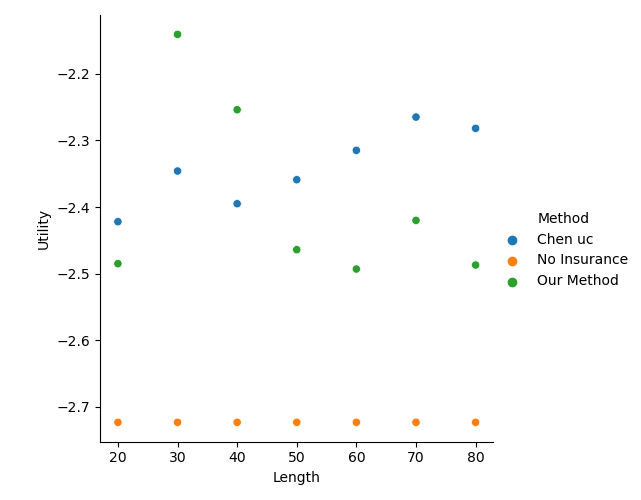
\includegraphics[width=0.6\textwidth]{../../../output/figures/Evaluation 2/Illinois_Utility_Length_ml1.png}
            \caption{Illinois Utility}
        \end{figure}
        \FloatBarrier

    \subsection{Insurer Cost}
        \begin{figure}[h]
            \centering
            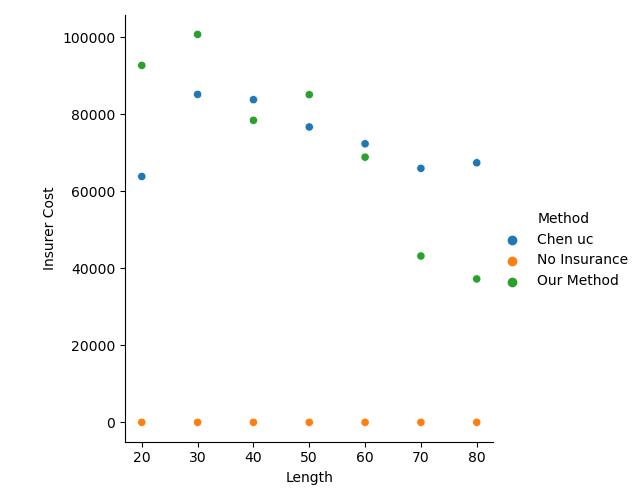
\includegraphics[width=0.6\textwidth]{../../../output/figures/Evaluation 2/Illinois_Insurer Cost_Length_ml1.png}
            \caption{Insurer Cost}
        \end{figure}
        \FloatBarrier

    \subsection{Over/Under Prediction Error}
        \begin{figure}[h]
            \centering
            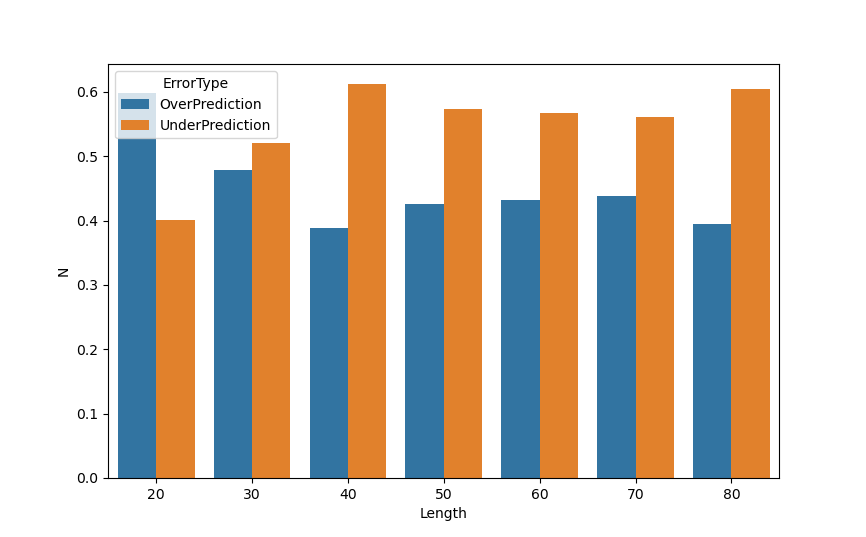
\includegraphics[width=0.6\textwidth]{../../../output/figures/Evaluation/Illinois_over_under_pred_error.png}
            \caption{Over/Under prediction errors}
        \end{figure}
        \FloatBarrier

\section{Other States Data Shortening}
  Our method outperforms Chen's method when evaluated on data from other states. There are some cases where our method opts for no insurance because it decides the farmer would be better off.  
    \subsection{Missouri Utility}
        \begin{figure}[h]
            \centering
            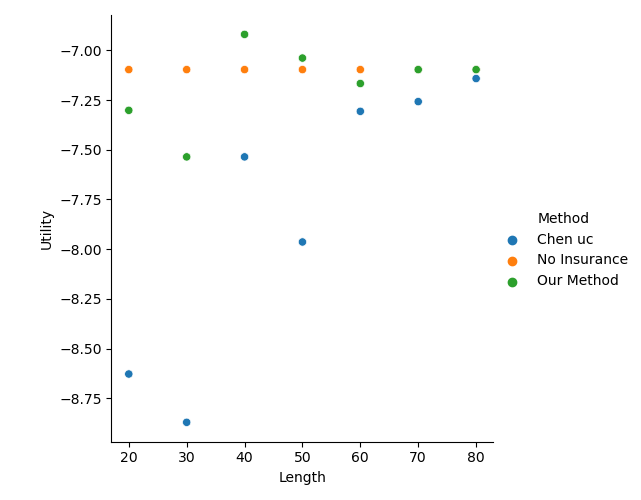
\includegraphics[width=0.6\textwidth]{../../../output/figures/Evaluation 2/Missouri_Utility_Length_ml1.png}
            \caption{Missouri Utility}
        \end{figure}
        \FloatBarrier

    \subsection{Iowa Utility}
    \begin{figure}[h]
        \centering
        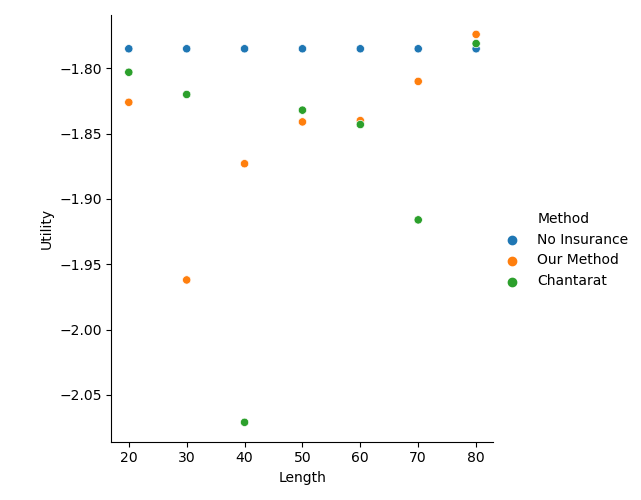
\includegraphics[width=0.6\textwidth]{../../../output/figures/Evaluation 2/Iowa_Utility_Length_ml1.png}
        \caption{Iowa Utility}
    \end{figure}
    \FloatBarrier

    \subsection{Indiana Utility}
        \begin{figure}[h]
            \centering
            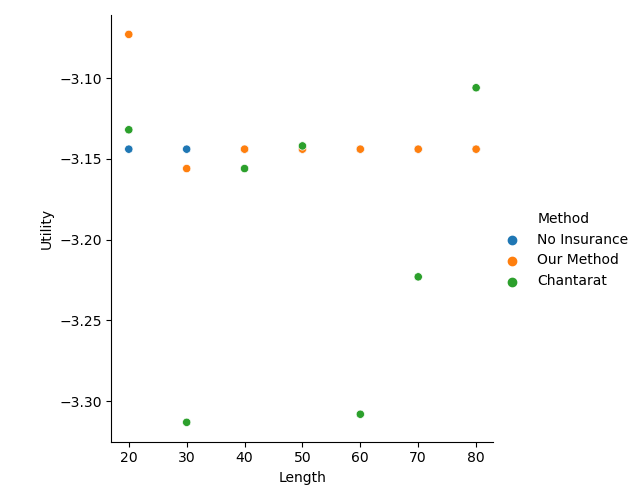
\includegraphics[width=0.6\textwidth]{../../../output/figures/Evaluation 2/Indiana_Utility_Length_ml1.png}
            \caption{Indiana Utility}
        \end{figure}
        \FloatBarrier
    
\section{Midwest Results}
  Our method consistently outperforms Chen's method in terms of overall utility and cost. It has a higher utility than Chen's method for every data length except the largest, and a lower cost in all but one length as well. Additionally, it leads to considerably lower capital requirements. When compared to our single zone method, the utility is slightly lower, but at lower costs and required capital. 
    \subsection{Overall Utility}
    \begin{figure}[h]
        \caption{Midwest Overall Utility}
        \centering
        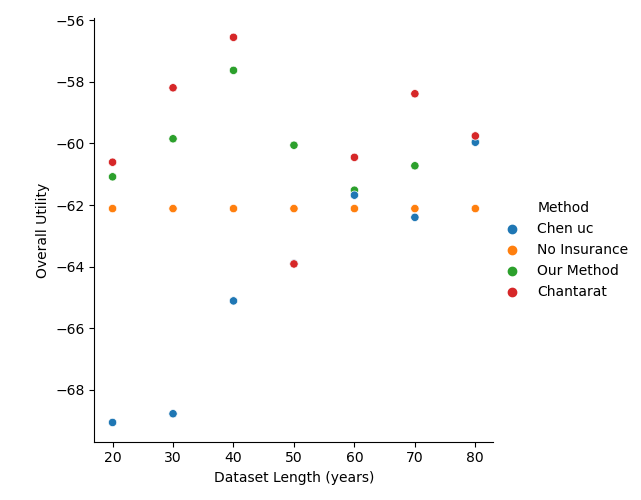
\includegraphics[width=0.6\textwidth]{../../../output/figures/Midwest Evaluation/Midwest_Overall Utility_Length.png}
        
    \end{figure}
    \FloatBarrier

    \subsection{Insurer Cost}
    \begin{figure}[h]
        \caption{Midwest Overall Insurer Cost}
    \centering
    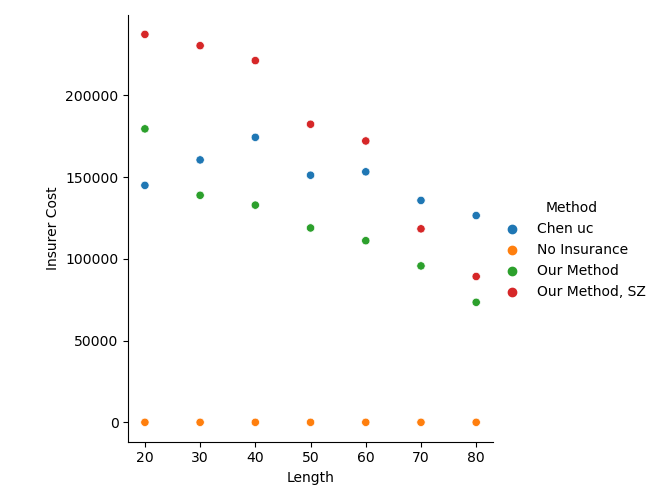
\includegraphics[width=0.6\textwidth]{../../../output/figures/Midwest Evaluation/Midwest_Insurer Cost_Length.png}
    
    \end{figure}
    \FloatBarrier

    \subsection{Required Capital}
    \begin{figure}[h]
        \caption{Midwest Overall Required Capital}
        \centering
        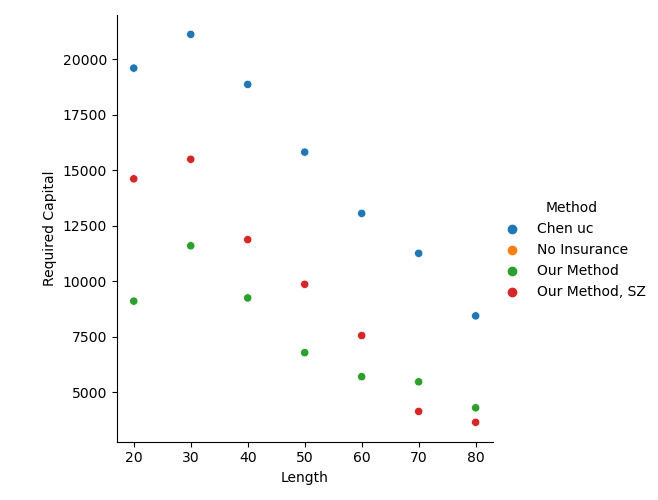
\includegraphics[width=0.6\textwidth]{../../../output/figures/Midwest Evaluation/Midwest_Required Capital_Length.png}
    \end{figure}
    \FloatBarrier

\section{Chen Premium Results}
  The results are fairly similar when using Chen's definition of the premium. In Illinois, our method outperforms Chen's method when there are 30-40 years of data. Our method consistently outperforms Chen's method when using data from Iowa and Missouri. Finally, the Indiana results are similar the Illinois results. 
    \subsection{Illinois Utility}
        \begin{figure}[h]
            \centering
            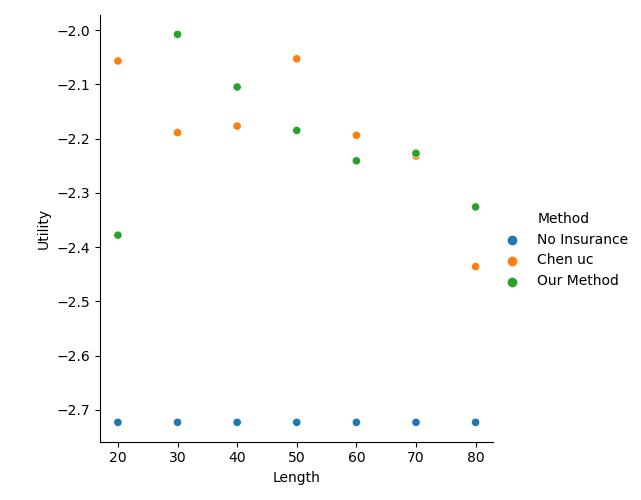
\includegraphics[width=0.6\textwidth]{../../../output/figures/Chen Premium/Illinois_Utility_Length_ml1241.png}
            \caption{Illinois Utility, Chen Premium}
        \end{figure}
        \FloatBarrier

    \subsection{Missouri Utility}
        \begin{figure}[h]
            \centering
            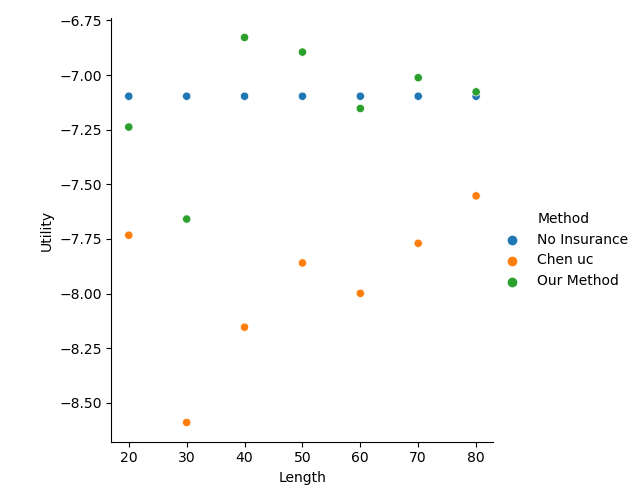
\includegraphics[width=0.6\textwidth]{../../../output/figures//Chen Premium/Missouri_Utility_Length_ml1241.png}
            \caption{Missouri Utility, Chen Premium}
        \end{figure}
        \FloatBarrier

    \subsection{Iowa Utility}
    \begin{figure}[h]
        \centering
        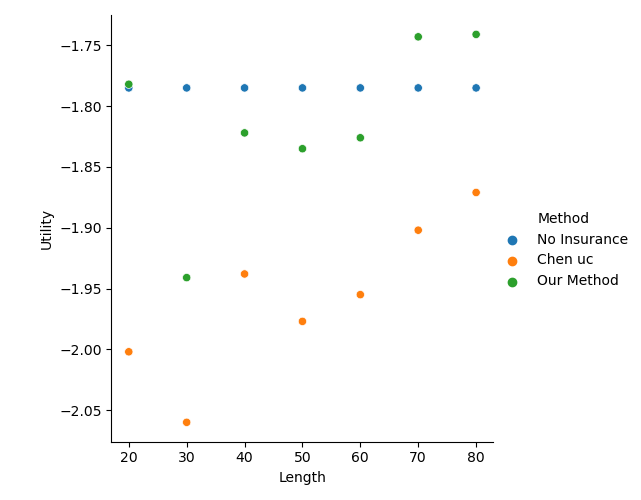
\includegraphics[width=0.6\textwidth]{../../../output/figures/Chen Premium/Iowa_Utility_Length_ml1241.png}
        \caption{Iowa Utility, Chen Premium}
    \end{figure}
    \FloatBarrier

    \subsection{Indiana Utility}
        \begin{figure}[h]
            \centering
            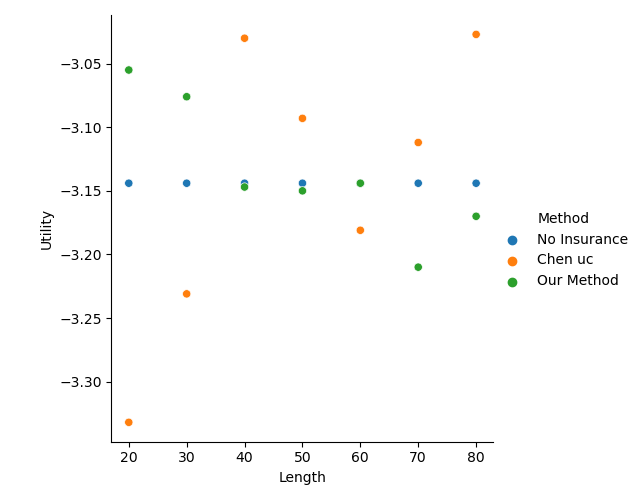
\includegraphics[width=0.6\textwidth]{../../../output/figures/Chen Premium/Indiana_Utility_Length_ml1241.png}
            \caption{Indiana Utility, Chen Premium}
        \end{figure}
        \FloatBarrier

\section{Potential Next Steps}
\begin{itemize}
  \item \textbf{Data shuffling:} We could re run the evaluation, but choose the train/validation and test set completely randomly. 
  \item \textbf{Regularization Exercise:} We could tune the regularization hyperparameter in Chen's method to show that it tends to overfit. 
  \item \textbf{Improve detrending:} We could improve the method used to de-trend the yield time-series. Chen used a second degree polynomial, however, locally weighted regression seems to work best according to the literature. 
  \item \textbf{Descriptive Analysis:} We could create plots to illustrate the difference between the two methods: 
    \begin{enumerate}
      \item Plot of payouts vs losses
      \item Distribution of farmer utility/wealth
      \item Distribution of insurer costs
      \item Distribution of insurer profits
      \item Plot illustrating in what cases farmer's are worse off with insurance
    \end{enumerate}
\end{itemize}
\end{document}